\begin{frame}[t,fragile]{Summary}
\begin{itemize}
  \item C++26 introduces significant improvements in the areas of:
  \begin{itemize}
    \mode<presentation>{\vfill\pause}
    \item \textmark{UB reduction and safety}: providing stronger guarantees against undefined behavior and improving the safety of C++ code.

    \mode<presentation>{\vfill\pause}
    \item \textmark{Reflection and compile-time programming}: enabling more powerful metaprogramming capabilities and allowing developers to write more efficient and expressive code.

    \mode<presentation>{\vfill\pause}
    \item \textmark{Contracts}: providing a standardized way to specify preconditions, postconditions, and invariants for functions and classes.

    \mode<presentation>{\vfill\pause}
    \item \textmark{Senders and receivers}: enabling a more flexible and composable approach to asynchronous programming.

    \mode<presentation>{\vfill\pause}
    \item \textmark{Parallelism support}: enhancing the standard library with new algorithms and utilities for parallel execution.
    
    \mode<presentation>{\vfill\pause}
    \item \textbad{And there is much more!}
  \end{itemize}
\end{itemize}
\end{frame}

\begin{frame}[t,fragile]{A final announcement}
\begin{center}
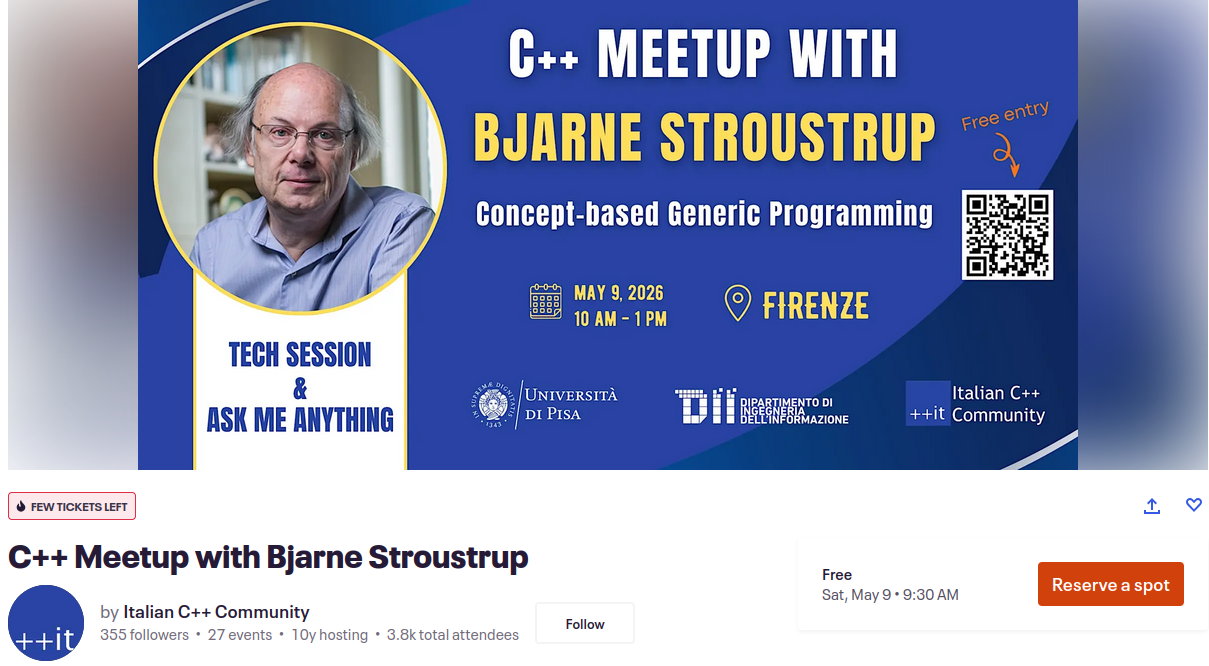
\includegraphics[height=0.8\textheight]{img/bjarne-firenze}
\textgood{\url{https://italiancpp-fi26.eventbrite.it/}}
\end{center}
\end{frame}